\documentclass[12pt]{article}
\usepackage{moodle}
\usepackage{fontspec}
\usepackage[brazilian]{babel}
%\usepackage[utf8]{inputenc}
%\usepackage[T1]{fontenc}
\usepackage{graphicx}
\ifwindows\imagemagickcommand{magick convert}
\else\imagemagickcommand{convert}
\fi

\begin{document}
	\begin{quiz}{Mudanças de Fase - Discursiva - Fácil}
		\begin{essay}[points=2,penalty=0,response format=file,attachments allowed=1,attachments required=1]{MDF01DF-40}
			Uma placa é atravessada por uma quantidade de calor igual a $3,0\times10^{3}$ cal em um intervalo de tempo de 5 minutos. Determine o fluxo de calor através dessa placa expressa em watt. Considere 1 cal = 4 J.	
		\end{essay}	
		\begin{essay}[points=2,penalty=0,response format=file,attachments allowed=1,attachments required=1]{MDF02DF-400}
			\textbf{(IME-RJ)} Um vidro plano, com coeficiente de condutibilidade térmica 0,00183 cal/s.cm.ºC, tem uma área de 1000 $cm^{2}$  e espessura de 3,66 mm. Sendo o fluxo de calor por condução através do vidro de 2000 cal/s, calcule a diferença de temperatura entre suas faces em ºC.
		\end{essay}
		\begin{essay}[points=2,penalty=0,response format=file,attachments allowed=1,attachments required=1]{MDF03DF-5/20}
			Uma barra de alumínio de 50 cm de comprimento e área de secção transversal de 5 $cm^{2}$  tem uma de suas extremidades em contato térmico com uma câmara de vapor de água em ebulição (100 ºC).  A outra extremidade está imersa em uma cuba que contém uma mistura bifásica de gelo fundente (0 ºC). A pressão atmosférica local é normal. Sabendo que o coeficiente de condutibilidade térmica do alumínio vale 0,5 cal/s.cm.ºC, calcule:\\
			a) o fluxo de calor através da barra, em cal/s, depois de estabelecido o regime permanente.\\
			b) a temperatura numa secção transversal da barra, em ºC, situada a 40 cm da extremidade mais quente.			
		\end{essay}
		\begin{essay}[points=2,penalty=0,response format=file,attachments allowed=1,attachments required=1]{MDF04DF-60}
			Na figura a seguir você observa uma placa de alumínio que foi utilizada para separar o interior de um forno, cuja temperatura mantinha-se estável a 220 ºC, e o meio ambiente (20 ºC). Após atingido o regime estacionário, qual a é o fluxo de calor, em kcal/s, através dessa chapa metálica? Suponha que o fluxo ocorra através da face de área maior. Dado: coeficiente de condutibilidade térmica do alumínio = 0,50 cal/s.cm.ºC.
			\begin{center}
				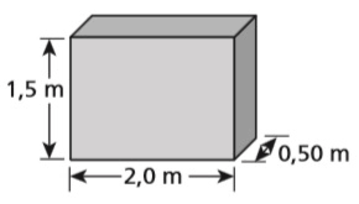
\includegraphics[width=0.7\linewidth]{img1.png}			
			\end{center}					
		\end{essay}
		\begin{essay}[points=2,penalty=0,response format=file,attachments allowed=1,attachments required=1]{MDF05DF-20}
			\textbf{(PUC MG/2014)}
			\begin{center}
			POTÊNCIA SOLAR
			\end{center}			
			O Sol emite uma enorme quantidade de energia da qual uma parte em um bilhão alcança a Terra. Não obstante, a quantidade de energia radiante recebida a cada segundo por metro quadrado perpendicular aos raios solares, no topo da atmosfera, é de 1400 joules (1,4 kJ).\\
			Essa quantidade de energia recebida a cada segundo por unidade de área é chamada de constante solar. Isso é equivalente em unidades de potência a 1,4 quilowatts por metro quadrado (1,4 $kW/m^{2}$). O valor da potência solar que atinge o solo é atenuado pela atmosfera e reduzida pelos ângulos de elevação solar não perpendiculares à superfície. Há também, é claro, a falta de luz durante a noite.\\
			A potência solar média recebida nos Estados Unidos, considerando-se dia e noite, verão e inverno, é cerca de 15\% da potência incidente nas partes altas da atmosfera.\\
			(Texto adaptado de HEWWITT. P. G. Física Conceitual. 9a Edição, 2002.)\\			
			Considerando-se um chuveiro elétrico com potência de 4200 W, calcule a área da superfície necessária, em $m^{2}$, no solo dos Estados Unidos, para suprir a potência desse equipamento com energia solar radiante.								
		\end{essay}										
	\end{quiz}
\end{document}